% supplement.tex -- Supplement 1 to manuscript.tex (JOSA A).
% Follows Optica's supplemental-document conventions: title "<article title>:
% supplemental document", no author block (Optica adds a cover sheet), and
% figures, tables, equations and sections numbered S1, S2, ... Every number is
% a numbers.tex macro; figures come from part2/code/figures/make_all.py.

\documentclass{optica-article}
\journal{opticajournal}
\articletype{Supplemental Document}
\usepackage{amsmath,booktabs}
% AUTO-GENERATED by scripts/make_numbers_tex.py -- DO NOT HAND-EDIT.
% Regenerate: python scripts/make_numbers_tex.py
\usepackage{xcolor}  % for the [PENDING] flag color, harmless if already loaded

\newcommand{\MeasuredContrastTwoX}{2.00}
\newcommand{\KcPredTwoX}{4.22}
\newcommand{\KstarTwoXInterp}{4.18}
\newcommand{\KstarTwoXCI}{\textcolor{red}{[PENDING]}}
\newcommand{\MeanGainTwoX}{0.40}
\newcommand{\MinGainTwoX}{-0.03}
\newcommand{\MeasuredContrastFourX}{3.80}
\newcommand{\KcPredFourX}{6.96}
\newcommand{\KstarFourXInterp}{\textcolor{red}{[PENDING]}}
\newcommand{\KstarFourXCI}{8.98}
\newcommand{\MeanGainFourX}{0.70}
\newcommand{\MinGainFourX}{0.04}
\newcommand{\MeasuredContrastEightX}{5.32}
\newcommand{\KcPredEightX}{9.33}
\newcommand{\KstarEightXInterp}{\textcolor{red}{[PENDING]}}
\newcommand{\KstarEightXCI}{8.98}
\newcommand{\MeanGainEightX}{0.88}
\newcommand{\MinGainEightX}{0.05}
\newcommand{\MinGainAllBudgets}{-0.03}
\newcommand{\SEightGainKLowSlantZero}{0.913}
\newcommand{\SEightLoKLowSlantZero}{0.906}
\newcommand{\SEightHiKLowSlantZero}{0.920}
\newcommand{\SEightGainKLowSlantTwoFive}{3.122}
\newcommand{\SEightLoKLowSlantTwoFive}{3.122}
\newcommand{\SEightHiKLowSlantTwoFive}{3.123}
\newcommand{\SEightGainKLowSlantFive}{2.077}
\newcommand{\SEightLoKLowSlantFive}{2.076}
\newcommand{\SEightHiKLowSlantFive}{2.078}
\newcommand{\SEightGainKLowSlantSevenFive}{0.227}
\newcommand{\SEightLoKLowSlantSevenFive}{0.223}
\newcommand{\SEightHiKLowSlantSevenFive}{0.230}
\newcommand{\SEightGainKLowSlantTen}{0.089}
\newcommand{\SEightLoKLowSlantTen}{0.089}
\newcommand{\SEightHiKLowSlantTen}{0.089}
\newcommand{\SEightGainKLowSlantFifteen}{-0.007}
\newcommand{\SEightLoKLowSlantFifteen}{-0.016}
\newcommand{\SEightHiKLowSlantFifteen}{0.002}
\newcommand{\SEightGainKLowSlantTwenty}{0.024}
\newcommand{\SEightLoKLowSlantTwenty}{0.019}
\newcommand{\SEightHiKLowSlantTwenty}{0.028}
\newcommand{\SEightGainKMidSlantZero}{0.899}
\newcommand{\SEightLoKMidSlantZero}{0.898}
\newcommand{\SEightHiKMidSlantZero}{0.901}
\newcommand{\SEightGainKMidSlantTwoFive}{1.017}
\newcommand{\SEightLoKMidSlantTwoFive}{0.980}
\newcommand{\SEightHiKMidSlantTwoFive}{1.055}
\newcommand{\SEightGainKMidSlantFive}{2.045}
\newcommand{\SEightLoKMidSlantFive}{2.044}
\newcommand{\SEightHiKMidSlantFive}{2.046}
\newcommand{\SEightGainKMidSlantSevenFive}{0.291}
\newcommand{\SEightLoKMidSlantSevenFive}{0.210}
\newcommand{\SEightHiKMidSlantSevenFive}{0.371}
\newcommand{\SEightGainKMidSlantTen}{0.185}
\newcommand{\SEightLoKMidSlantTen}{0.182}
\newcommand{\SEightHiKMidSlantTen}{0.187}
\newcommand{\SEightGainKMidSlantFifteen}{0.046}
\newcommand{\SEightLoKMidSlantFifteen}{0.045}
\newcommand{\SEightHiKMidSlantFifteen}{0.046}
\newcommand{\SEightGainKMidSlantTwenty}{0.011}
\newcommand{\SEightLoKMidSlantTwenty}{0.011}
\newcommand{\SEightHiKMidSlantTwenty}{0.011}
\newcommand{\NZZeroPooledGainThirtyTwo}{0.640}
\newcommand{\NZZeroPooledLoThirtyTwo}{0.640}
\newcommand{\NZZeroPooledHiThirtyTwo}{0.640}
\newcommand{\NZZeroPooledGainOneTwentyEight}{0.641}
\newcommand{\NZZeroPooledLoOneTwentyEight}{0.641}
\newcommand{\NZZeroPooledHiOneTwentyEight}{0.641}
\newcommand{\NZZeroPooledGainTwoFiftySix}{0.645}
\newcommand{\NZZeroPooledLoTwoFiftySix}{0.645}
\newcommand{\NZZeroPooledHiTwoFiftySix}{0.645}
\newcommand{\NZZeroGainKLowThirtyTwo}{1.019}
\newcommand{\NZZeroGainKLowOneTwentyEight}{0.915}
\newcommand{\NZZeroGainKLowTwoFiftySix}{0.894}
\newcommand{\NZZeroGainKMidThirtyTwo}{0.731}
\newcommand{\NZZeroGainKMidOneTwentyEight}{0.900}
\newcommand{\NZZeroGainKMidTwoFiftySix}{0.928}
\newcommand{\SOneBaselineGain}{1.81}
\newcommand{\SOneNoSaturationGain}{2.22}
\newcommand{\SOneNoSaturationRatio}{1.2}
\newcommand{\SOneNoDiffusionRatio}{1.14}
\newcommand{\SOneNoNonlocalityRatio}{0.98}
\newcommand{\SOneNoDyeDepletionRatio}{0.98}
\newcommand{\STwoBaselineGain}{0.11}
\newcommand{\STwoGainMin}{0.08}
\newcommand{\STwoGainMax}{0.15}
\newcommand{\SThreeNominalGain}{1.81}
\newcommand{\SThreeWorstWithinFifty}{1.17}
\newcommand{\SThreeWorstWithinFiftyParam}{dn\_max}
\newcommand{\SThreeBestWithinFifty}{1.92}
\newcommand{\SThreeDnMaxFlipPct}{473}
\newcommand{\SThreeDnMaxWorstGain}{-3.73}
\newcommand{\SThreeDnMaxAtHundred}{0.99}
\newcommand{\SThreeDnMaxMostNegativePct}{-83}
\newcommand{\SThreeDnMaxAtMostNegative}{0.38}
\newcommand{\SThreeDnMaxMostPositivePct}{473}
\newcommand{\SThreeDnMaxAtMostPositive}{-3.73}
\newcommand{\SThreeAnyFlipWithinFifty}{no}
\newcommand{\SATMeanGainTwoX}{0.07}
\newcommand{\SATFracOfMILTwoX}{18}
\newcommand{\SATMeanGainFourX}{0.20}
\newcommand{\SATFracOfMILFourX}{28}
\newcommand{\SATMeanGainEightX}{0.36}
\newcommand{\SATFracOfMILEightX}{42}
\newcommand{\SATFitNRMSE}{0.103}
\newcommand{\SATFitAEff}{7.05}
\newcommand{\SATSubCliffGain}{0.98}
\newcommand{\SATSubCliffMILGain}{1.37}
\newcommand{\SATSubCliffFracOfMIL}{71}
\newcommand{\SATSubCliffFracMin}{79}
\newcommand{\SATSubCliffFracMax}{79}
\newcommand{\SATSubCliffK}{1.31}
\newcommand{\SATNearCliffK}{3.93}
\newcommand{\SATNearCliffFrac}{56}
\newcommand{\SATPostCliffK}{5.24}
\newcommand{\SATPostCliffFracMin}{-28}
\newcommand{\SATPostCliffFracMax}{-28}
\newcommand{\SeedCountMin}{3}
\newcommand{\SeedCountMax}{3}
\newcommand{\SeedCountDesc}{3}
\newcommand{\SeedCountModal}{3}
\newcommand{\SeedCountNExtraConfigs}{0}
\newcommand{\SeedCount}{3}
\newcommand{\NResultFiles}{2375}

% --- supplement macros (already-real data, not Phase-3-gated) ---
\newcommand{\AblationCheckpointCosSim}{1.000}
\newcommand{\AblationSurrogateCosSim}{0.844}
\newcommand{\RCWAMaxDevThreeCase}{0.038}
\newcommand{\RCWAVGridMaxDev}{0.980}
\newcommand{\RCWAVGridNCases}{90}
\newcommand{\RCWAUnslantedMaxDev}{0.29}
\newcommand{\RCWANormalMedianDev}{0.001}
\newcommand{\MeshPSNRSpread}{0.036}
\newcommand{\WavelengthDesignPSNR}{6.63}

% --- validation (Phase 6 / Section 6) macros ---
\newcommand{\NLiteratureSources}{3}
\newcommand{\NRMSEBruderGrowthDnKExp}{0.28}
\newcommand{\NRMSEBruderGrowthDnKSim}{0.17}
\newcommand{\NRMSEHsiehGrowthDnK}{0.10}
\newcommand{\NRMSEWorstFit}{0.28}
\newcommand{\NRMSEBestFit}{0.10}
\newcommand{\NGoodFits}{3}
\newcommand{\NRMSEWorstInRegime}{0.28}
\newcommand{\NRMSEBestInRegime}{0.17}
\newcommand{\NInRegimeSources}{2}
\newcommand{\BayfolDnMaxRatio}{5.7}

% --- baseline completeness (Sec. 5.2 / F4b) macros ---
\newcommand{\GSGainMin}{-1.27}
\newcommand{\GSGainMax}{0.00}
\newcommand{\LPCGainMin}{-1.82}
\newcommand{\LPCGainMax}{0.07}
\newcommand{\MILGainMinAtTwoX}{-0.03}

% --- shrinkage-induced shift bound (Discussion) macros ---
\newcommand{\ShrinkagePct}{0.5}
\newcommand{\ShrinkageSlantDeg}{20}
\newcommand{\ShrinkageThicknessUm}{30}
\newcommand{\ShrinkageShiftNm}{54.6}
\newcommand{\ShrinkageFracLowK}{1.7}
\newcommand{\ShrinkageFracHighK}{13.7}

% --- cost-benefit (Sec. 5.1) macros ---
\newcommand{\ComputeMatchRatio}{21.7}

% --- R1 reconstruction figure macros ---
\newcommand{\ROneSeedValue}{0}

% --- WP3 baseline (RSGD/GPC, Sec. 5.2) macros ---
\newcommand{\RSGDGainMin}{-0.00}
\newcommand{\RSGDGainMax}{0.00}
\newcommand{\GPCGainMin}{-1.98}
\newcommand{\GPCGainMax}{0.07}
\newcommand{\GPCLPCMaxAbsDiffTwoX}{0.18}

% --- WP4 (target ensemble / noise robustness, Sec. 5.x) macros ---
\newcommand{\SFourGainBarsTwoX}{0.90}
\newcommand{\SFourBootCILoBarsTwoX}{0.90}
\newcommand{\SFourBootCIHiBarsTwoX}{0.90}
\newcommand{\SFourGainBarsEightX}{1.95}
\newcommand{\SFourBootCILoBarsEightX}{1.95}
\newcommand{\SFourBootCIHiBarsEightX}{1.95}
\newcommand{\SFourGainSpotsTwoX}{3.22}
\newcommand{\SFourBootCILoSpotsTwoX}{3.19}
\newcommand{\SFourBootCIHiSpotsTwoX}{3.23}
\newcommand{\SFourGainSpotsEightX}{4.07}
\newcommand{\SFourBootCILoSpotsEightX}{3.99}
\newcommand{\SFourBootCIHiSpotsEightX}{4.12}
\newcommand{\SFourGainRandomBinaryTwoX}{0.17}
\newcommand{\SFourBootCILoRandomBinaryTwoX}{0.17}
\newcommand{\SFourBootCIHiRandomBinaryTwoX}{0.17}
\newcommand{\SFourGainRandomBinaryEightX}{0.24}
\newcommand{\SFourBootCILoRandomBinaryEightX}{0.24}
\newcommand{\SFourBootCIHiRandomBinaryEightX}{0.24}
\newcommand{\SFiveNoiseStdPct}{5}
\newcommand{\SFiveNoiselessGain}{0.90}
\newcommand{\SFiveNoisyGain}{0.88}

% --- WP5 (joint miscalibration Monte Carlo, Sec. 5.x) macros ---
\newcommand{\SSixNDraws}{30}
\newcommand{\SSixMeanGain}{1.76}
\newcommand{\SSixBootCILo}{1.73}
\newcommand{\SSixBootCIHi}{1.79}
\newcommand{\SSixNNegative}{0}
\newcommand{\SSixWorstDrawGain}{1.61}
\newcommand{\SSixBestDrawGain}{1.94}
\newcommand{\SSixPctRange}{25}

% --- WP6 (depth-resolved absorption, Sec. 5.x) macros ---
\newcommand{\SSevenGainODZero}{1.81}
\newcommand{\SSevenGainODOneTenth}{1.51}
\newcommand{\SSevenGainODThreeTenths}{1.45}

% --- PATH_TO_7 rewrite macros (complete M1 cells only) ---
\newcommand{\MOneNK}{10}
\newcommand{\MOneNCells}{30}
\newcommand{\MOneKMin}{1.96}
\newcommand{\MOneKMax}{15.71}
\newcommand{\MOneKList}{1.96, 2.62, 3.49, 3.93, 4.19, 4.83, 5.71, 6.98, 8.98, 15.71}
\newcommand{\MOneNPositive}{29}
\newcommand{\MOneNCIAboveZero}{27}
\newcommand{\MOneNCIIncludesZero}{2}
\newcommand{\MOneNNegative}{1}
\newcommand{\MOneNegK}{4.19}
\newcommand{\MOneNegBudget}{2}
\newcommand{\MOneNegGain}{-0.03}
\newcommand{\MOneNegCILo}{-0.05}
\newcommand{\MOneNegCIHi}{-0.005}
\newcommand{\MaxGainTwoX}{1.42}
\newcommand{\MaxGainKTwoX}{2.62}
\newcommand{\GainHighKTwoX}{0.01}
\newcommand{\GainHighKLoTwoX}{0.002}
\newcommand{\GainHighKHiTwoX}{0.008}
\newcommand{\MaxGainFourX}{2.13}
\newcommand{\MaxGainKFourX}{1.96}
\newcommand{\GainHighKFourX}{0.04}
\newcommand{\GainHighKLoFourX}{0.009}
\newcommand{\GainHighKHiFourX}{0.062}
\newcommand{\MaxGainEightX}{2.52}
\newcommand{\MaxGainKEightX}{2.62}
\newcommand{\GainHighKEightX}{0.05}
\newcommand{\GainHighKLoEightX}{0.019}
\newcommand{\GainHighKHiEightX}{0.091}
\newcommand{\MOneNExcluded}{0}
\newcommand{\SOneGBaselineSub}{4.41}
\newcommand{\SOneGBaselineNear}{0.90}
\newcommand{\SOneGBaselinePost}{0.11}
\newcommand{\SOneGNoSatSub}{5.39}
\newcommand{\SOneGNoSatNear}{0.61}
\newcommand{\SOneGNoSatPost}{0.66}
\newcommand{\SOneGNoDiffSub}{4.93}
\newcommand{\SOneGNoDiffNear}{1.14}
\newcommand{\SOneGNoDiffPost}{0.10}
\newcommand{\SOneGNoNonlocSub}{4.47}
\newcommand{\SOneGNoNonlocNear}{0.82}
\newcommand{\SOneGNoNonlocPost}{0.05}
\newcommand{\SOneGNoDyeSub}{4.36}
\newcommand{\SOneGNoDyeNear}{0.84}
\newcommand{\SOneGNoDyePost}{0.11}
\newcommand{\SOneKSub}{1.31}
\newcommand{\SOneKNear}{3.93}
\newcommand{\SOneKPost}{5.24}
\newcommand{\SXGBaselineSub}{4.41}
\newcommand{\SXNBaselineSub}{3}
\newcommand{\SXGBaselineNear}{0.90}
\newcommand{\SXNBaselineNear}{3}
\newcommand{\SXGBaselinePost}{0.11}
\newcommand{\SXNBaselinePost}{3}
\newcommand{\SXGNoMonomerSub}{-0.12}
\newcommand{\SXNNoMonomerSub}{3}
\newcommand{\SXGNoMonomerNear}{-0.09}
\newcommand{\SXNNoMonomerNear}{3}
\newcommand{\SXGNoMonomerPost}{-0.08}
\newcommand{\SXNNoMonomerPost}{3}
\newcommand{\SXGNoDyeSub}{4.35}
\newcommand{\SXNNoDyeSub}{3}
\newcommand{\SXGNoDyeNear}{0.84}
\newcommand{\SXNNoDyeNear}{3}
\newcommand{\SXGNoDyePost}{0.11}
\newcommand{\SXNNoDyePost}{3}
\newcommand{\SXGNoSatSub}{5.38}
\newcommand{\SXNNoSatSub}{3}
\newcommand{\SXGNoSatNear}{0.62}
\newcommand{\SXNNoSatNear}{3}
\newcommand{\SXGNoSatPost}{0.66}
\newcommand{\SXNNoSatPost}{3}
\newcommand{\SXGOnlyTanhSub}{-0.10}
\newcommand{\SXNOnlyTanhSub}{3}
\newcommand{\SXGOnlyTanhNear}{-0.02}
\newcommand{\SXNOnlyTanhNear}{3}
\newcommand{\SXGOnlyTanhPost}{-0.03}
\newcommand{\SXNOnlyTanhPost}{3}
\newcommand{\SXGOnlyDyeSub}{14.37}
\newcommand{\SXNOnlyDyeSub}{3}
\newcommand{\SXGOnlyDyeNear}{6.38}
\newcommand{\SXNOnlyDyeNear}{3}
\newcommand{\SXGOnlyDyePost}{7.40}
\newcommand{\SXNOnlyDyePost}{3}
\newcommand{\SXGOnlyMonomerSub}{5.75}
\newcommand{\SXNOnlyMonomerSub}{3}
\newcommand{\SXGOnlyMonomerNear}{1.73}
\newcommand{\SXNOnlyMonomerNear}{3}
\newcommand{\SXGOnlyMonomerPost}{1.26}
\newcommand{\SXNOnlyMonomerPost}{3}
\newcommand{\SXGLinearSub}{14.94}
\newcommand{\SXNLinearSub}{3}
\newcommand{\SXGLinearNear}{7.66}
\newcommand{\SXNLinearNear}{3}
\newcommand{\SXGLinearPost}{9.04}
\newcommand{\SXNLinearPost}{3}
\newcommand{\SXGLinearMatchedSub}{-0.00}
\newcommand{\SXNLinearMatchedSub}{3}
\newcommand{\SXGLinearMatchedNear}{0.00}
\newcommand{\SXNLinearMatchedNear}{3}
\newcommand{\SXGLinearMatchedPost}{0.10}
\newcommand{\SXNLinearMatchedPost}{3}
\newcommand{\SXGNoMonomerMatchedSub}{3.64}
\newcommand{\SXNNoMonomerMatchedSub}{3}
\newcommand{\SXGNoMonomerMatchedNear}{0.72}
\newcommand{\SXNNoMonomerMatchedNear}{3}
\newcommand{\SXGNoMonomerMatchedPost}{0.08}
\newcommand{\SXNNoMonomerMatchedPost}{3}
\newcommand{\SXGOnlyDyeMatchedSub}{1.98}
\newcommand{\SXNOnlyDyeMatchedSub}{3}
\newcommand{\SXGOnlyDyeMatchedNear}{0.42}
\newcommand{\SXNOnlyDyeMatchedNear}{3}
\newcommand{\SXGOnlyDyeMatchedPost}{-0.02}
\newcommand{\SXNOnlyDyeMatchedPost}{3}
\newcommand{\SXGOnlyTanhMatchedSub}{2.80}
\newcommand{\SXNOnlyTanhMatchedSub}{3}
\newcommand{\SXGOnlyTanhMatchedNear}{0.53}
\newcommand{\SXNOnlyTanhMatchedNear}{3}
\newcommand{\SXGOnlyTanhMatchedPost}{0.12}
\newcommand{\SXNOnlyTanhMatchedPost}{3}
\newcommand{\SXDeviceMaxDiff}{0.001}
\newcommand{\SATFracLowKMin}{36}
\newcommand{\SATFracLowKMax}{44}
\newcommand{\SATFracSecondKMin}{53}
\newcommand{\SATFracSecondKMax}{66}
\newcommand{\SATNBelowBSGD}{12}
\newcommand{\SATNCells}{29}
\newcommand{\SThreeDnMaxAtMinusFifty}{1.17}
\newcommand{\SThreeDnMaxAtPlusFifty}{1.66}
\newcommand{\MTwoRGainSub}{3.19}
\newcommand{\MTwoRLoSub}{2.94}
\newcommand{\MTwoRHiSub}{3.43}
\newcommand{\MTwoRGainNear}{0.81}
\newcommand{\MTwoRLoNear}{0.81}
\newcommand{\MTwoRHiNear}{0.81}
\newcommand{\MTwoRGainPost}{0.12}
\newcommand{\MTwoRLoPost}{0.12}
\newcommand{\MTwoRHiPost}{0.13}
\newcommand{\MTwoRSATFracSub}{79}
\newcommand{\MTwoRSATFracNear}{56}
\newcommand{\MTwoRSATFracPost}{-28}
\newcommand{\HoldoutASimIn}{0.17}
\newcommand{\HoldoutASimOut}{0.48}
\newcommand{\HoldoutASimKbleach}{\textcolor{red}{[PENDING]}}
\newcommand{\HoldoutASimDnMax}{0.0504}
\newcommand{\HoldoutASimAtBound}{none}
\newcommand{\HoldoutAExpIn}{0.28}
\newcommand{\HoldoutAExpOut}{1.09}
\newcommand{\HoldoutAExpKbleach}{\textcolor{red}{[PENDING]}}
\newcommand{\HoldoutAExpDnMax}{0.289}
\newcommand{\HoldoutAExpAtBound}{none}
\newcommand{\HoldoutBSimIn}{0.02}
\newcommand{\HoldoutBSimOut}{0.40}
\newcommand{\HoldoutBSimKbleach}{0.0667}
\newcommand{\HoldoutBSimDnMax}{0.0418}
\newcommand{\HoldoutBSimAtBound}{none}
\newcommand{\HoldoutBExpIn}{0.17}
\newcommand{\HoldoutBExpOut}{0.31}
\newcommand{\HoldoutBExpKbleach}{0.0215}
\newcommand{\HoldoutBExpDnMax}{0.0321}
\newcommand{\HoldoutBExpAtBound}{none}

% --- diffraction-efficiency confirmation (Sec. 5.1) macros ---
\newcommand{\DEMeanGainTwoX}{1.80}
\newcommand{\DEMeanGainFourX}{3.00}
\newcommand{\DEMeanGainEightX}{3.94}
\newcommand{\DEMinGainAllBudgets}{-0.251}
\newcommand{\DENNegative}{15}
\newcommand{\DENPairs}{90}

% --- wasted-media measurement (Sec. 5.4) macros ---
\newcommand{\WastedMediaThreshDB}{2}
\newcommand{\WastedMediaBSGDFrac}{37}
\newcommand{\WastedMediaMILFrac}{0}
\newcommand{\WastedMediaBSGDFracOneDB}{60}
\newcommand{\WastedMediaMILFracOneDB}{57}
\newcommand{\WastedMediaBSGDFracThreeDB}{17}
\newcommand{\WastedMediaMILFracThreeDB}{0}
\newcommand{\WastedMediaNConfigs}{30}
\newcommand{\WastedMediaGSFrac}{53}
\newcommand{\WastedMediaGSFracOneDB}{60}
\newcommand{\WastedMediaGSFracThreeDB}{33}
\newcommand{\WastedMediaLPCFrac}{47}
\newcommand{\WastedMediaLPCFracOneDB}{60}
\newcommand{\WastedMediaLPCFracThreeDB}{33}
\newcommand{\WastedMediaSATFrac}{33}
\newcommand{\WastedMediaSATFracOneDB}{60}
\newcommand{\WastedMediaSATFracThreeDB}{0}
\newcommand{\WastedMediaRSGDFrac}{37}
\newcommand{\WastedMediaRSGDFracOneDB}{60}
\newcommand{\WastedMediaRSGDFracThreeDB}{17}
\newcommand{\WastedMediaGPCFrac}{47}
\newcommand{\WastedMediaGPCFracOneDB}{60}
\newcommand{\WastedMediaGPCFracThreeDB}{30}


\renewcommand{\thesection}{S\arabic{section}}
\renewcommand{\thefigure}{S\arabic{figure}}
\renewcommand{\thetable}{S\arabic{table}}
\renewcommand{\theequation}{S\arabic{equation}}
\renewcommand{\topfraction}{0.9}
\renewcommand{\textfraction}{0.07}
\renewcommand{\floatpagefraction}{0.8}

\begin{document}

\title{Media-in-the-loop holography: designing photopolymer exposures through a
differentiable recording model: supplemental document}

\begin{abstract*}
This document supports the main article with the heuristic small-signal
analysis behind the $K_c$ prediction, the full mechanism ablations, the
slice-count and slant tables, the miscalibration, compute-matched, target and
noise studies, the RCWA check of the closed-form readout, the twin fits with the
dye-bleaching rate held, implementation checks, and a map from every reported
result to the files and scripts that produce it. Section, figure and table
numbers without an ``S'' refer to the main article.
\end{abstract*}

% ----------------------------------------------------------------------
\section{Heuristic small-signal transfer function and $K_c$}
\label{sec:s1}
\textbf{Derivation.} Take $I(x)=I_{\text{mean}}(1+m\cos Kx)$ with $m\ll1$,
neglect dye depletion ($d\approx1$) and hold $D_{\text{eff}}=D_0$, i.e.\
linearize Eqs.~(2)--(4) about the start of recording. The uniform fields obey
$\dot u_0=-F_0u_0$ with $F_0=\kappa I_{\text{mean}}^\gamma$. Eliminating the
first-order Fourier component quasi-statically gives
\begin{equation}
H(K)=\frac{\exp(-K^2\sigma^2/2)}{1+D_0K^2/F_0},
\label{eq:hk}
\end{equation}
implemented as \texttt{NPDDRecorder.small\_signal\_mtf} in the released code. A
compensation limit follows if the pre-boost $1/H(K)$ needed to undo the
roll-off exceeds the contrast budget.

\textbf{Status.} Equation~(\ref{eq:hk}) does not match the full simulator, while
an independent numerical linearization of the same equations does. $H(K)$ is
therefore a heuristic that motivated the hypothesis, not a validated transfer
function, and no result depends on its being exact. LPC (Section~3), which
uses it directly, improves on media-blind SGD by at most \LPCGainMax\,dB.

\textbf{Definition of $K_c$.} The pipeline compares $1/H(K)$ with the contrast
the optimizer actually realized at each grid $K$, not the nominal budget, and
reports the smallest $K$ at which $1/H$ exceeds it, by linear interpolation.
The mean realized contrast is \MeasuredContrastTwoX, \MeasuredContrastFourX{}
and \MeasuredContrastEightX{} at nominal budgets 2, 4 and 8, giving
$K_c=\KcPredTwoX$, \KcPredFourX{} and \KcPredEightX\,rad/\textmu m. At budget 8
the optimizer does not realize the nominal contrast at several $K$, which is
why $K_c$ grows less than the nominal budget would suggest. The observed zero
crossing exists only at budget 2 ($K^*=\KstarTwoXInterp$\,rad/\textmu m).

\textbf{Exposures and index profiles behind Fig.~2.} Figure~\ref{fig:s1}
shows the exposures $E(x)$ and recorded index profiles $\Delta n(x)$ of the
reconstructions in Fig.~2. In these single-seed examples the linear assumption
drives BSGD's exposure toward near-binary swings between zero and the contrast
cap, which at the higher $K$ push $\Delta n(x)$ toward $\Delta n_{\max}$ over
most of the period; MIL's exposure is less extreme at the lowest $K$. This is an
illustration of one seed, not a statistical claim.

\begin{figure}[!htbp]
\centering
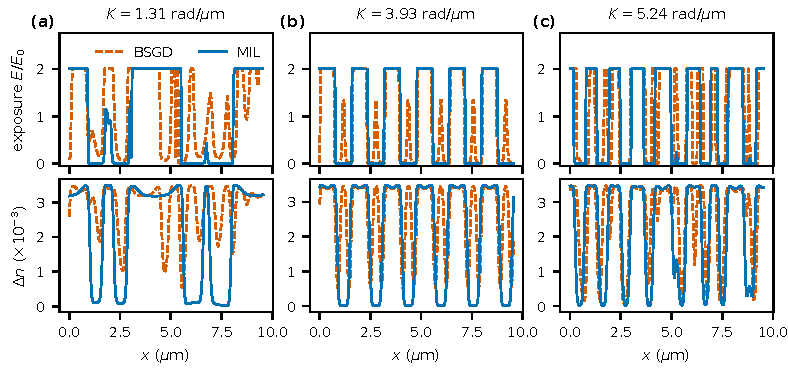
\includegraphics[width=\linewidth]{../code/figures/paper/FigS1_exposure_profiles.pdf}
\caption{Exposure $E/E_0$ (top) and recorded $\Delta n$ (bottom) for BSGD and
MIL, same $K$, budget $B_c=2$, seed and $9.6\,\mu$m section as Fig.~2.}
\label{fig:s1}
\end{figure}

% ----------------------------------------------------------------------
\section{Mechanism ablations}
\label{sec:s2}
\textbf{One mechanism at a time.} The conditions are $\sigma\to0$ (no
non-locality), $D_0\to0$ (no diffusion), $k_{\text{bleach}}\to0$ (no dye
bleaching), and the $\tanh$ index map replaced by its linear limit
$\Delta n=1.5\,\Delta n_{\max}N$ (no index saturation). Table~3 lists the means;
Fig.~\ref{fig:s2} adds the intervals.

\begin{figure}[!htbp]
\centering
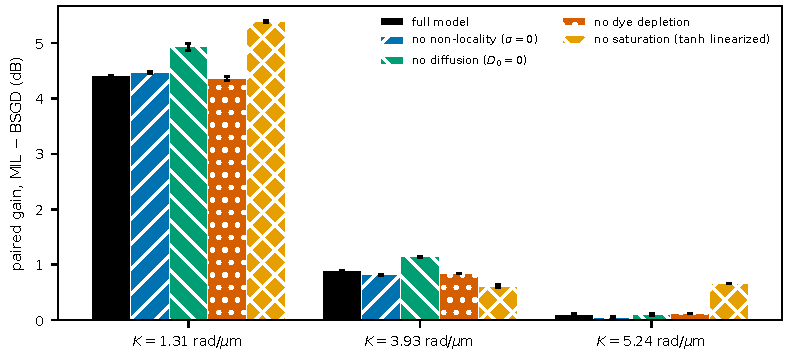
\includegraphics[width=\linewidth]{../code/figures/paper/FigS2_ablation.pdf}
\caption{Paired gain with one mechanism removed at three $K$, $B_c=2$, 95\%
$t$-intervals over three seeds.}
\label{fig:s2}
\end{figure}

\textbf{Factorial over the saturating mechanisms.} M denotes monomer depletion
(removed by holding $u\equiv1$: polymer production continues at the local rate
and the reservoir never empties), D dye bleaching ($k_{\text{bleach}}=0$ when
removed) and T the $\tanh$ index map (linearized when removed).
``Matched'' rows rescale $\kappa$ so that the polymer cured at unit uniform dose
is $N=1$, as in the full model: $\kappa=0.2/(1-e^{-2})$ with bleaching and
$\kappa=0.1$ without. ``Linear, slope-matched'' sets $\kappa=1/15$ with all
three removed, so that $\Delta n=\Delta n_{\max}(G_\sigma*E)$, the media-blind
model up to blur and shrinkage. The factorial ran on CPU (single precision); its
full-model row reproduces the GPU values of Table~3 to within
\SXDeviceMaxDiff\,dB. Table~\ref{tab:s1} lists every condition and
Fig.~\ref{fig:s3} shows the intervals.

\begin{table}[!htbp]
\centering
\caption{Paired gain (dB) for every factorial condition, $B_c=2$, mean of
three seeds. Active mechanisms: M monomer depletion, D dye bleaching, T $\tanh$
map.}
\label{tab:s1}
\renewcommand{\arraystretch}{1.15}
\begin{tabular}{llccc}
\toprule
Active & Condition & $K=\SOneKSub$ & $K=\SOneKNear$ & $K=\SOneKPost$ \\
\midrule
M D T & full model & \SXGBaselineSub & \SXGBaselineNear & \SXGBaselinePost \\
D T & no monomer depletion & \SXGNoMonomerSub & \SXGNoMonomerNear & \SXGNoMonomerPost \\
D T & \quad matched & \SXGNoMonomerMatchedSub & \SXGNoMonomerMatchedNear & \SXGNoMonomerMatchedPost \\
M T & no dye bleaching & \SXGNoDyeSub & \SXGNoDyeNear & \SXGNoDyePost \\
M D & no index saturation & \SXGNoSatSub & \SXGNoSatNear & \SXGNoSatPost \\
T & only $\tanh$ & \SXGOnlyTanhSub & \SXGOnlyTanhNear & \SXGOnlyTanhPost \\
T & \quad matched & \SXGOnlyTanhMatchedSub & \SXGOnlyTanhMatchedNear & \SXGOnlyTanhMatchedPost \\
D & only dye bleaching & \SXGOnlyDyeSub & \SXGOnlyDyeNear & \SXGOnlyDyePost \\
D & \quad matched & \SXGOnlyDyeMatchedSub & \SXGOnlyDyeMatchedNear & \SXGOnlyDyeMatchedPost \\
M & only monomer depletion & \SXGOnlyMonomerSub & \SXGOnlyMonomerNear & \SXGOnlyMonomerPost \\
-- & linear & \SXGLinearSub & \SXGLinearNear & \SXGLinearPost \\
-- & linear, slope-matched & \SXGLinearMatchedSub & \SXGLinearMatchedNear & \SXGLinearMatchedPost \\
\bottomrule
\end{tabular}
\end{table}

\textbf{Unmatched conditions.} Without operating-point matching, removing
monomer depletion with the $\tanh$ map kept saturates the map almost everywhere,
and both methods then fail equally (gains \SXGNoMonomerSub,
\SXGNoMonomerNear{} and \SXGNoMonomerPost\,dB; ``only $\tanh$'' behaves the
same way). With the map linearized as well (``only dye bleaching'',
``linear''), the cured polymer and hence the index modulation are an order of
magnitude deeper than BSGD's linear model assumes, and the large gains
(\SXGLinearSub, \SXGLinearNear{} and \SXGLinearPost\,dB for ``linear'') measure
that modulation-depth mismatch rather than saturation. This is why the main
text compares only operating-point-matched conditions.

\begin{figure}[!htbp]
\centering
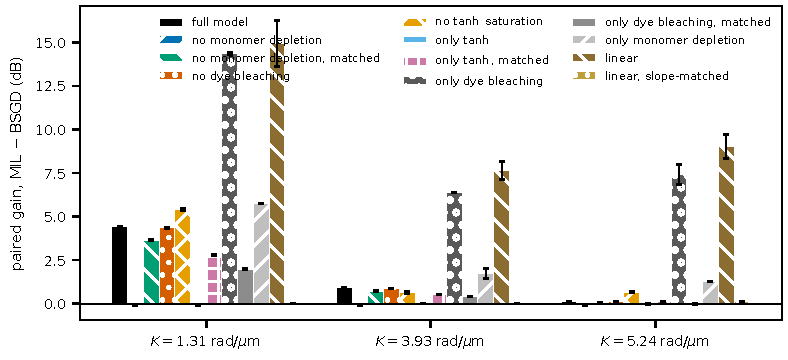
\includegraphics[width=\linewidth]{../code/figures/paper/FigS3_factorial.pdf}
\caption{Paired gain for every factorial condition of Table~\ref{tab:s1}, three
$K$, $B_c=2$, 95\% $t$-intervals over seeds.}
\label{fig:s3}
\end{figure}

% ----------------------------------------------------------------------
\section{Readout slice count and grating slant}
\label{sec:s3}
Table~\ref{tab:s2} gives the paired gain for $n_z=32$, 128 and 256 (one seed,
$B_c=2$, unslanted). All experiments use $n_z=128$; $n_z=32$ is not converged at
$K=3.93$\,rad/\textmu m. Table~\ref{tab:s3} gives the slant dependence of
Fig.~3(a) with intervals. The slanted values rely on the scalar readout outside
the geometry in which it was checked against RCWA (Section~\ref{sec:s5}) and
are model-dependent.

\begin{table}[!htbp]
\centering
\caption{Paired gain (dB) versus number of readout slices $n_z$, one seed.}
\label{tab:s2}
\begin{tabular}{lccc}
\toprule
$K$ (rad/\textmu m) & $n_z=32$ & $n_z=128$ & $n_z=256$ \\
\midrule
1.96 & \NZZeroGainKLowThirtyTwo & \NZZeroGainKLowOneTwentyEight & \NZZeroGainKLowTwoFiftySix \\
3.93 & \NZZeroGainKMidThirtyTwo & \NZZeroGainKMidOneTwentyEight & \NZZeroGainKMidTwoFiftySix \\
pooled over three $K$ & \NZZeroPooledGainThirtyTwo & \NZZeroPooledGainOneTwentyEight & \NZZeroPooledGainTwoFiftySix \\
\bottomrule
\end{tabular}
\end{table}

\begin{table}[!htbp]
\centering
\caption{Paired gain (dB) versus grating slant $\phi$, $B_c=2$, mean of three
seeds with 95\% $t$-interval.}
\label{tab:s3}
\small
\setlength{\tabcolsep}{3pt}
\begin{tabular}{lccccccc}
\toprule
$\phi$ & $0^\circ$ & $2.5^\circ$ & $5^\circ$ & $7.5^\circ$ & $10^\circ$ & $15^\circ$ & $20^\circ$ \\
\midrule
$K=1.96$ & \SEightGainKLowSlantZero & \SEightGainKLowSlantTwoFive & \SEightGainKLowSlantFive & \SEightGainKLowSlantSevenFive & \SEightGainKLowSlantTen & \SEightGainKLowSlantFifteen & \SEightGainKLowSlantTwenty \\
 & {\scriptsize[\SEightLoKLowSlantZero, \SEightHiKLowSlantZero]} & {\scriptsize[\SEightLoKLowSlantTwoFive, \SEightHiKLowSlantTwoFive]} & {\scriptsize[\SEightLoKLowSlantFive, \SEightHiKLowSlantFive]} & {\scriptsize[\SEightLoKLowSlantSevenFive, \SEightHiKLowSlantSevenFive]} & {\scriptsize[\SEightLoKLowSlantTen, \SEightHiKLowSlantTen]} & {\scriptsize[\SEightLoKLowSlantFifteen, \SEightHiKLowSlantFifteen]} & {\scriptsize[\SEightLoKLowSlantTwenty, \SEightHiKLowSlantTwenty]} \\
$K=3.93$ & \SEightGainKMidSlantZero & \SEightGainKMidSlantTwoFive & \SEightGainKMidSlantFive & \SEightGainKMidSlantSevenFive & \SEightGainKMidSlantTen & \SEightGainKMidSlantFifteen & \SEightGainKMidSlantTwenty \\
 & {\scriptsize[\SEightLoKMidSlantZero, \SEightHiKMidSlantZero]} & {\scriptsize[\SEightLoKMidSlantTwoFive, \SEightHiKMidSlantTwoFive]} & {\scriptsize[\SEightLoKMidSlantFive, \SEightHiKMidSlantFive]} & {\scriptsize[\SEightLoKMidSlantSevenFive, \SEightHiKMidSlantSevenFive]} & {\scriptsize[\SEightLoKMidSlantTen, \SEightHiKMidSlantTen]} & {\scriptsize[\SEightLoKMidSlantFifteen, \SEightHiKMidSlantFifteen]} & {\scriptsize[\SEightLoKMidSlantTwenty, \SEightHiKMidSlantTwenty]} \\
\bottomrule
\end{tabular}
\end{table}

% ----------------------------------------------------------------------
\section{One-parameter miscalibration}
\label{sec:s4}
Both exposures are designed on the nominal twin and recorded, unchanged, on a
twin with one of $D_0$, $\sigma$, $\kappa$ or $\Delta n_{\max}$ perturbed, at
$K=\SOneKSub$, \SOneKNear{} and \SOneKPost\,rad/\textmu m, $B_c=2$; the gain is
averaged over $K$ for each seed and the 95\% interval is taken over seeds
(Fig.~3(b)). Within $\pm50\%$ the gain stays between \SThreeWorstWithinFifty{}
and \SThreeBestWithinFifty\,dB, the lowest value belonging to $\Delta n_{\max}$
at $-50\%$ (nominal \SThreeNominalGain\,dB). For $\Delta n_{\max}$ the sweep is
extended to bracket the \BayfolDnMaxRatio$\times$ disagreement between the two
Bayfol fits with $k_{\text{bleach}}$ held (Section~\ref{sec:s9}): the gain is
\SThreeDnMaxAtMostNegative\,dB at $\SThreeDnMaxMostNegativePct\%$,
\SThreeDnMaxAtMinusFifty\,dB at $-50\%$, \SThreeDnMaxAtPlusFifty\,dB at
$+50\%$, \SThreeDnMaxAtHundred\,dB at $+100\%$ and
\SThreeDnMaxAtMostPositive\,dB at $+\SThreeDnMaxMostPositivePct\%$. The grid has
no points between $+100\%$ and $+\SThreeDnMaxMostPositivePct\%$, so where the sign
changes is not resolved. BSGD's design depends on the medium only through the
scale $\Delta n_{\max}$ of its linear model, so its exposure is the same at
every perturbation; the change in paired gain reflects how MIL's design and both
recordings respond to the error.

% ----------------------------------------------------------------------
\section{RCWA check of the closed-form readout}
\label{sec:s5}
Kogelnik first-order efficiency~\cite{kogelnik1969coupled} was compared with
RCWA~\cite{moharam1981rigorous}, computed with TORCWA~\cite{kim2023torcwa}. A
three-case check (TE, unslanted, near Bragg incidence) agrees to
\RCWAMaxDevThreeCase{} in absolute efficiency. Over the
\RCWAVGridNCases-case grid (TE and TM, three geometries, several $\Delta n$ and
$K$) the deviation is at most \RCWAUnslantedMaxDev{} for unslanted geometries,
with median \RCWANormalMedianDev{} at normal incidence, and up to
\RCWAVGridMaxDev{} for a $20^\circ$ slant, where the slant detunes the Bragg
condition (Fig.~\ref{fig:s4}). This checks the closed-form reference rather than
the beam propagation inside the design loop; the two share the scalar
approximation, which is why the headline claims are restricted to unslanted
gratings.

\begin{figure}[!htbp]
\centering
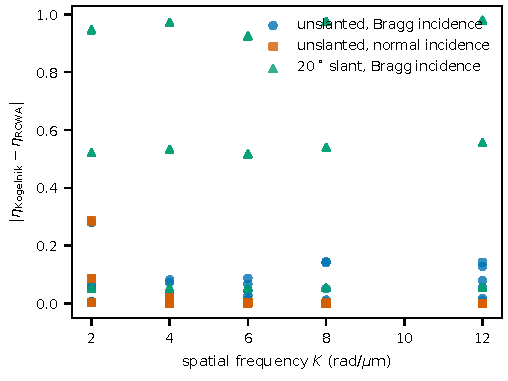
\includegraphics[width=0.62\linewidth]{../code/figures/paper/FigS4_rcwa_envelope.pdf}
\caption{Absolute deviation of Kogelnik first-order efficiency from RCWA over
the \RCWAVGridNCases-case grid, one series per geometry.}
\label{fig:s4}
\end{figure}

% ----------------------------------------------------------------------
\section{Compute-matched control}
\label{sec:s6}
BSGD receives $\lceil 800\times\ComputeMatchRatio\rceil$ iterations and MIL
keeps 800. The ratio is one wall-clock measurement of per-iteration cost, not a
FLOP count. The control was run at $B_c=2$ only, three seeds, three $K$
(Table~\ref{tab:s4}); the last row gives the saturation-only surrogate's gain as
a percentage of MIL's at the same points.

\begin{table}[!htbp]
\centering
\caption{Compute-matched paired gain (dB), $B_c=2$.}
\label{tab:s4}
\begin{tabular}{lccc}
\toprule
 & $K=\SOneKSub$ & $K=\SOneKNear$ & $K=\SOneKPost$ \\
\midrule
MIL $-$ BSGD (compute-matched) & \MTwoRGainSub & \MTwoRGainNear & \MTwoRGainPost \\
95\% interval & [\MTwoRLoSub, \MTwoRHiSub] & [\MTwoRLoNear, \MTwoRHiNear] & [\MTwoRLoPost, \MTwoRHiPost] \\
MIL $-$ BSGD (equal iterations) & \SOneGBaselineSub & \SOneGBaselineNear & \SOneGBaselinePost \\
SAT as \% of MIL & \MTwoRSATFracSub & \MTwoRSATFracNear & \MTwoRSATFracPost \\
\bottomrule
\end{tabular}
\end{table}

% ----------------------------------------------------------------------
\section{Calibrating the twin for a new medium}
\label{sec:s7}
From the fits of Section~5 and Section~\ref{sec:s9}: (i) $\kappa$ and
$\Delta n_{\max}$ are identifiable from one $\Delta n_1$(dose) curve;
(ii) $D_0$ and $\sigma$ act through the spatial-frequency dependence and need a
multi-$K$ family or an independent measurement, so a single-$K$ curve should
not be used to fit them; (iii) $\Delta n_{\max}$ must come from the same
experimental condition as the curve being fitted, not from a separate
experiment on the same material; (iv) the dose-to-time mapping and
$k_{\text{bleach}}$ are coupled, so $k_{\text{bleach}}$ should be fitted (as in
Section~5) or the source intensity recovered; holding it at an assumed value
can make the fit degenerate (Section~\ref{sec:s9}).

% ----------------------------------------------------------------------
\section{Target content and readout noise}
\label{sec:s8}
At $K=3.93$\,rad/\textmu m, three target families (bars, sparse random spots,
random binary), budgets 2 and 8, three seeds, with bootstrap 95\%
intervals~\cite{efron1993bootstrap} (Table~\ref{tab:s5}). Gaussian detector
noise at \SFiveNoiseStdPct\% of the reconstructed peak, applied identically to
every method before scoring, changes the bar-target gain from
\SFiveNoiselessGain{} to \SFiveNoisyGain\,dB ($B_c=2$). With three seeds the
bootstrap intervals are coarse; they are reported alongside, not instead of,
the $t$-intervals used elsewhere.

\begin{table}[!htbp]
\centering
\caption{Paired gain (dB) by target family at $K=3.93$\,rad/\textmu m, with
bootstrap 95\% intervals.}
\label{tab:s5}
\begin{tabular}{lcc}
\toprule
Target & $B_c=2$ & $B_c=8$ \\
\midrule
bars & \SFourGainBarsTwoX{} [\SFourBootCILoBarsTwoX, \SFourBootCIHiBarsTwoX] & \SFourGainBarsEightX{} [\SFourBootCILoBarsEightX, \SFourBootCIHiBarsEightX] \\
sparse spots & \SFourGainSpotsTwoX{} [\SFourBootCILoSpotsTwoX, \SFourBootCIHiSpotsTwoX] & \SFourGainSpotsEightX{} [\SFourBootCILoSpotsEightX, \SFourBootCIHiSpotsEightX] \\
random binary & \SFourGainRandomBinaryTwoX{} [\SFourBootCILoRandomBinaryTwoX, \SFourBootCIHiRandomBinaryTwoX] & \SFourGainRandomBinaryEightX{} [\SFourBootCILoRandomBinaryEightX, \SFourBootCIHiRandomBinaryEightX] \\
\bottomrule
\end{tabular}
\end{table}

% ----------------------------------------------------------------------
\section{Twin fits with the dye-bleaching rate held}
\label{sec:s9}
Figure~\ref{fig:s5} shows the fits with only $\kappa$ and $\Delta n_{\max}$ free
and $k_{\text{bleach}}=0.2$ held (best of ten random starts). For the Bayfol HX
model curve the fit reproduces the rise and decline (NRMSE
\NRMSEBruderGrowthDnKSim). For the measured series the optimum (NRMSE
\NRMSEBruderGrowthDnKExp) is degenerate: the fitted $\kappa$ saturates the medium
before the first measured dose, so the twin returns an almost constant
$\Delta n_1$, and the fitted $\Delta n_{\max}$ (\HoldoutAExpDnMax) is
\BayfolDnMaxRatio$\times$ that of the model-curve fit (\HoldoutASimDnMax).
Freeing $k_{\text{bleach}}$ removes the degeneracy (Fig.~4). The PQ/PMMA curve
of Hsieh et al.~\cite{hsieh2022pqpmma} is the source's own kinetic-model output
at $K=24.94$\,rad/\textmu m, outside the tested range, and is still rising at the
end of the record, so $\Delta n_{\max}$ is under-constrained; its fit (NRMSE
\NRMSEHsiehGrowthDnK) is not used as evidence in the main text.

\begin{figure}[!htbp]
\centering
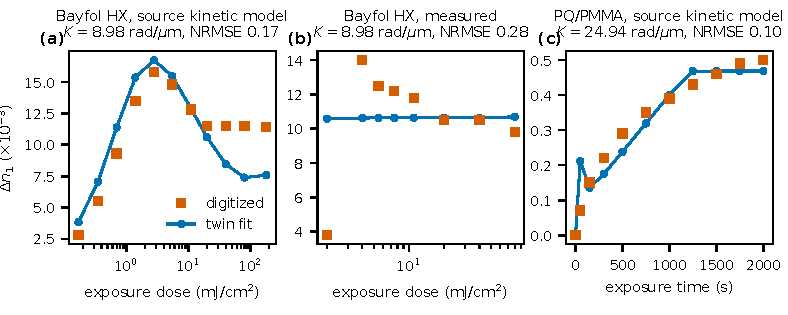
\includegraphics[width=\linewidth]{../code/figures/paper/FigS5_twin_fits_held_kbleach.pdf}
\caption{Twin fits with $k_{\text{bleach}}=0.2$ held: (a) Bayfol HX model
curve and (b) measurement~\cite{bruder2017bayfol}; (c) PQ/PMMA model
curve~\cite{hsieh2022pqpmma}, outside the tested $K$ range.}
\label{fig:s5}
\end{figure}

% ----------------------------------------------------------------------
\section{Implementation checks}
\label{sec:s10}
\textbf{Non-local kernel.} The kernel $G_\sigma$ is applied to the production
term $Fu$ (polymer initiated at $x'$ is deposited at $x$), not to $u$ alone, as
the NPDD model requires~\cite{sheridan2000nonlocal}.

\textbf{Conservation.} The explicit reaction step caps consumed monomer at the
monomer available, so $u\ge0$ and $u+N$ is conserved to rounding error at any
step size.

\textbf{Gradients.} At the configuration of the main grid ($n_x=1024$,
300 integrator steps, $n_z=128$, default medium, $B_c=2$, bar target at
$K=3.93$\,rad/\textmu m, float64), the directional derivative of the loss from
reverse-mode differentiation through the full chain (softplus, projection,
recording, beam propagation, loss) agrees with a central finite difference
along \GradCheckNDirs{} random unit directions to a maximum relative error of
$\GradCheckMaxRelErr$ (\texttt{experiments/gradient\_check.py}; the test
exposure is kept below the contrast cap so the projection is smooth there).

\textbf{Reproducibility.} Each per-job result file records its configuration,
the git commit of the code that produced it and the device; the seed enters only
through the optimizer initialization.

% ----------------------------------------------------------------------
\section{Provenance of reported results}
\label{sec:s11}
Every number in the main article and this supplement is a macro in
\texttt{numbers.tex}, generated by \texttt{scripts/make\_numbers\_tex.py}
(with \texttt{analysis/de\_confirmation.py} and
\texttt{analysis/wasted\_media.py}) from the per-job result files in
\texttt{results/}, one JSON file per tier, configuration, method and seed,
aggregated by \texttt{analysis/aggregate.py}. Figures are generated by
\texttt{figures/make\_all.py}. Table~\ref{tab:s6} maps each result to its
source; paths are relative to \texttt{part2/code/} of the released repository,
and \texttt{REPRODUCE.md} there lists the commands.

\begin{table}[!htbp]
\centering
\caption{Source of each reported result.}
\label{tab:s6}
\small
\renewcommand{\arraystretch}{1.15}
\begin{tabularx}{\linewidth}{>{\raggedright\arraybackslash}p{0.36\linewidth} X}
\toprule
Result & Tier and source \\
\midrule
Paired gain on the grid, Fig.~1(a), failure rates (Table~2), diffraction efficiency & M1; \texttt{aggregate.py}, \texttt{wasted\_media.py}, \texttt{de\_confirmation.py} \\
Baselines and SAT, Fig.~1(b) & M1 \\
Reconstructions and profiles, Figs.~2 and S1 & \texttt{experiments/make\_r1\_reconstructions.py}, \texttt{make\_r1\_profiles.py} \\
Compute-matched control & M2R \\
Ablations and factorial, Table~3, Tables~S1, Figs.~S2--S3 & S1, S1X \\
Slant and slice count, Fig.~3(a), Tables~S2--S3 & S8, NZ0 \\
Miscalibration, joint draws, depth absorption, Fig.~3(b) & S3, S6, S7 (\texttt{experiments/run\_s3\_mismatch.py}, \texttt{run\_s6\_joint\_mismatch.py}, \texttt{run\_s7\_depth\_absorption.py}) \\
Re-optimized parameter sensitivity & S2R \\
Targets and noise, Table~S5 & S4, S5 \\
Twin fits and held-out prediction, Figs.~4 and S5 & \texttt{experiments/fit\_literature\_curves.py}, \texttt{fit\_twin\_holdout.py}; digitized data in \texttt{data/literature/} \\
RCWA check, Fig.~S4 & \texttt{experiments/rcwa\_crosscheck.py} \\
Medium and simulation parameters (Table~1) & \texttt{experiments/manifest.py}, \texttt{configs/media/} \\
\bottomrule
\end{tabularx}
\end{table}

\bibliography{refs}

\end{document}
